\section{RESULTADOS}\label{cap:results}

\subsection{Estructura de los Resultados}\label{sec:results}

En este capítulo se presentan los resultados de la investigación mostrada en Metodología~\ref{cap:metodologia}. Se ha dividido en dos partes, la primera muestra los resultados del Estudio 1 y la segunda los resultados del Estudio 2.

\subsection{Resultados del Estudio 1}\label{sec:resultados-estudio-1}

\subsubsection{Frecuencia Cardíaca}

A continuación, se muestra el análisis de la varianza realizado para la \textit{Frecuencia Cardíaca}, la \textit{Frecuencia Cardíaca Escalada} y la \textit{Frecuencia Cardíaca Transformada por Cuantiles} entre pacientes que sufren DETERIORO y los que no. Se ha realizado el análisis de la varianza para cada una de las medias horarias. El resultado se muestra en la Tabla~\ref{tab:mean-FC}.  


\begin{table}[H]
    \centering
    \begin{tabular}{|c|r|r|r|}
        \hline
        \textbf{Media Horaria} & \textbf{p-valor} & \textbf{p-valor 
        cuantiles} & \textbf{p-valor 
        escalada} \\
        \hline
        MEAN\_1 & 0.129 & 0.142 & 0.902 \\
        MEAN\_2 & 0.254 & 0.412 & 0.825 \\
        MEAN\_3 & 0.143 & 0.105 & 0.925 \\
        MEAN\_4 & 0.331 & 0.309 & 0.867 \\
        MEAN\_5 & 0.077 & 0.042 & 0.355 \\
        MEAN\_6 & 0.098 & 0.1 & 0.5 \\
        MEAN\_7 & 0.357 & 0.232 & 0.474 \\
        MEAN\_8 & 0.182 & 0.218 & 0.975 \\
        MEAN\_9 & 0.158 & 0.241 & 0.83 \\
        MEAN\_10 & 0.316 & 0.423 & 0.211 \\
        MEAN\_11 & 0.609 & 0.637 & 0.045 \\
        MEAN\_12 & 0.035 & 0.005 & 0.382 \\
        MEAN\_13 & 0.293 & 0.144 & 0.603 \\
        MEAN\_14 & 0.169 & 0.17 & 0.727 \\
        MEAN\_15 & 0.214 & 0.335 & 0.722 \\
        MEAN\_16 & 0.094 & 0.136 & 0.652 \\
        MEAN\_17 & 0.127 & 0.132 & 0.943 \\
        MEAN\_18 & 0.476 & 0.816 & 0.56 \\
        MEAN\_19 & 0.128 & 0.086 & 0.731 \\
        MEAN\_20 & 0.2 & 0.186 & 0.947 \\
        MEAN\_21 & 0.391 & 0.592 & 0.643 \\
        MEAN\_22 & 0.157 & 0.198 & 0.875 \\
        MEAN\_23 & 0.1 & 0.026 & 0.445 \\
        MEAN\_24 & 0.204 & 0.187 & 0.95 \\
        \hline
    \end{tabular}
    \caption{p-valor de la media horaria de la \textit{Frecuencia Cardíaca} y la \textit{Frecuencia Cardíaca Transformada por Cuantiles} entre pacientes que sufren OAF y los que no}\label{tab:mean-FC}
\end{table}

De manera gráfica el resultado es el siguiente mostrado en la Figura~\ref{fig:mean-FC}. Se han añadido dos rectas verticales que muestran el nivel del valor $\alpha$ = 0.05 y $\alpha$ = 0.001. ($\alpha$ = 0.01 se excluye del gráfico ya que a pesar de ser un nivel de significancia ampliamente utilizado, haría que el gráfico se viese peor al amontonarse las líneas verticales en la parte inferior de la imagen). Se puede observar que la mayoría de las medias horarias no son significativas, por lo que no se puede rechazar la hipótesis nula. Esto significa que no hay diferencias significativas entre las medias horarias de la \textit{Frecuencia Cardíaca} entre pacientes que sufren DETERIORO y los que no.

Se puede observar como de manera general que a los pacientes que se les suministra OAF tienen una mayor \textit{Frecuencia Cardíaca} que los que no. Esto se puede observar en la Figura~\ref{fig:fc-boxplot-mean}, aun así no se puede afirmar que esto tenga un efecto significativo de manera general en toda la monitorización del paciente.

Las medias más significativas son las referentes a las horas 12 y 23. Esta situación va a causar a la hora de realizar el \textit{Estudio 2} se tendrán problemas a la hora de realizar un modelo de clasificación dónde los valores de monitorización de la \textit{Frecuencia Cardíaca} sean significativos a la hora de clasificar pacientes como DETERIORO o no.

\begin{figure}[H]
    \centering
    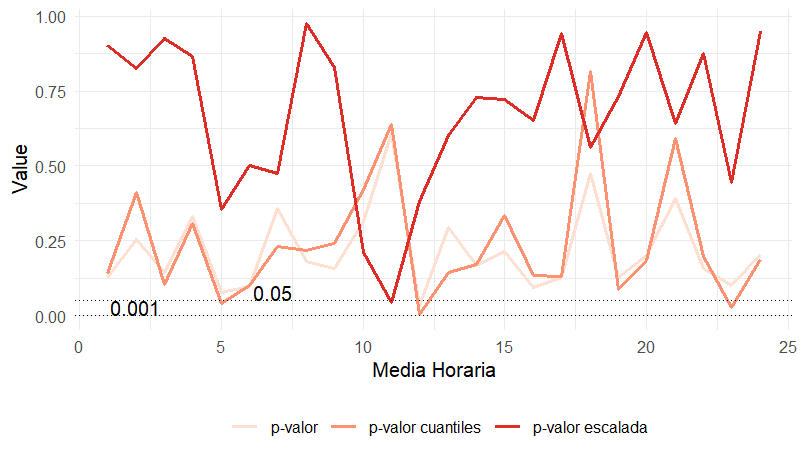
\includegraphics[scale = 1]{./img/mean-FC.png}
    \caption{p-valor de la media horaria de la \textit{Frecuencia Cardíaca} entre pacientes que sufren DETERIORO y los que no}
    \label{fig:mean-FC}
\end{figure}

\newpage
\thispagestyle{empty}
% Se modifica la geometría (los márgenes) de la página y se coloca en formato horizontal:
\newgeometry{top=10mm, bottom=10mm, left=12mm, right=12mm}
\begin{landscape}
\begin{figure}[H]
    \centering
    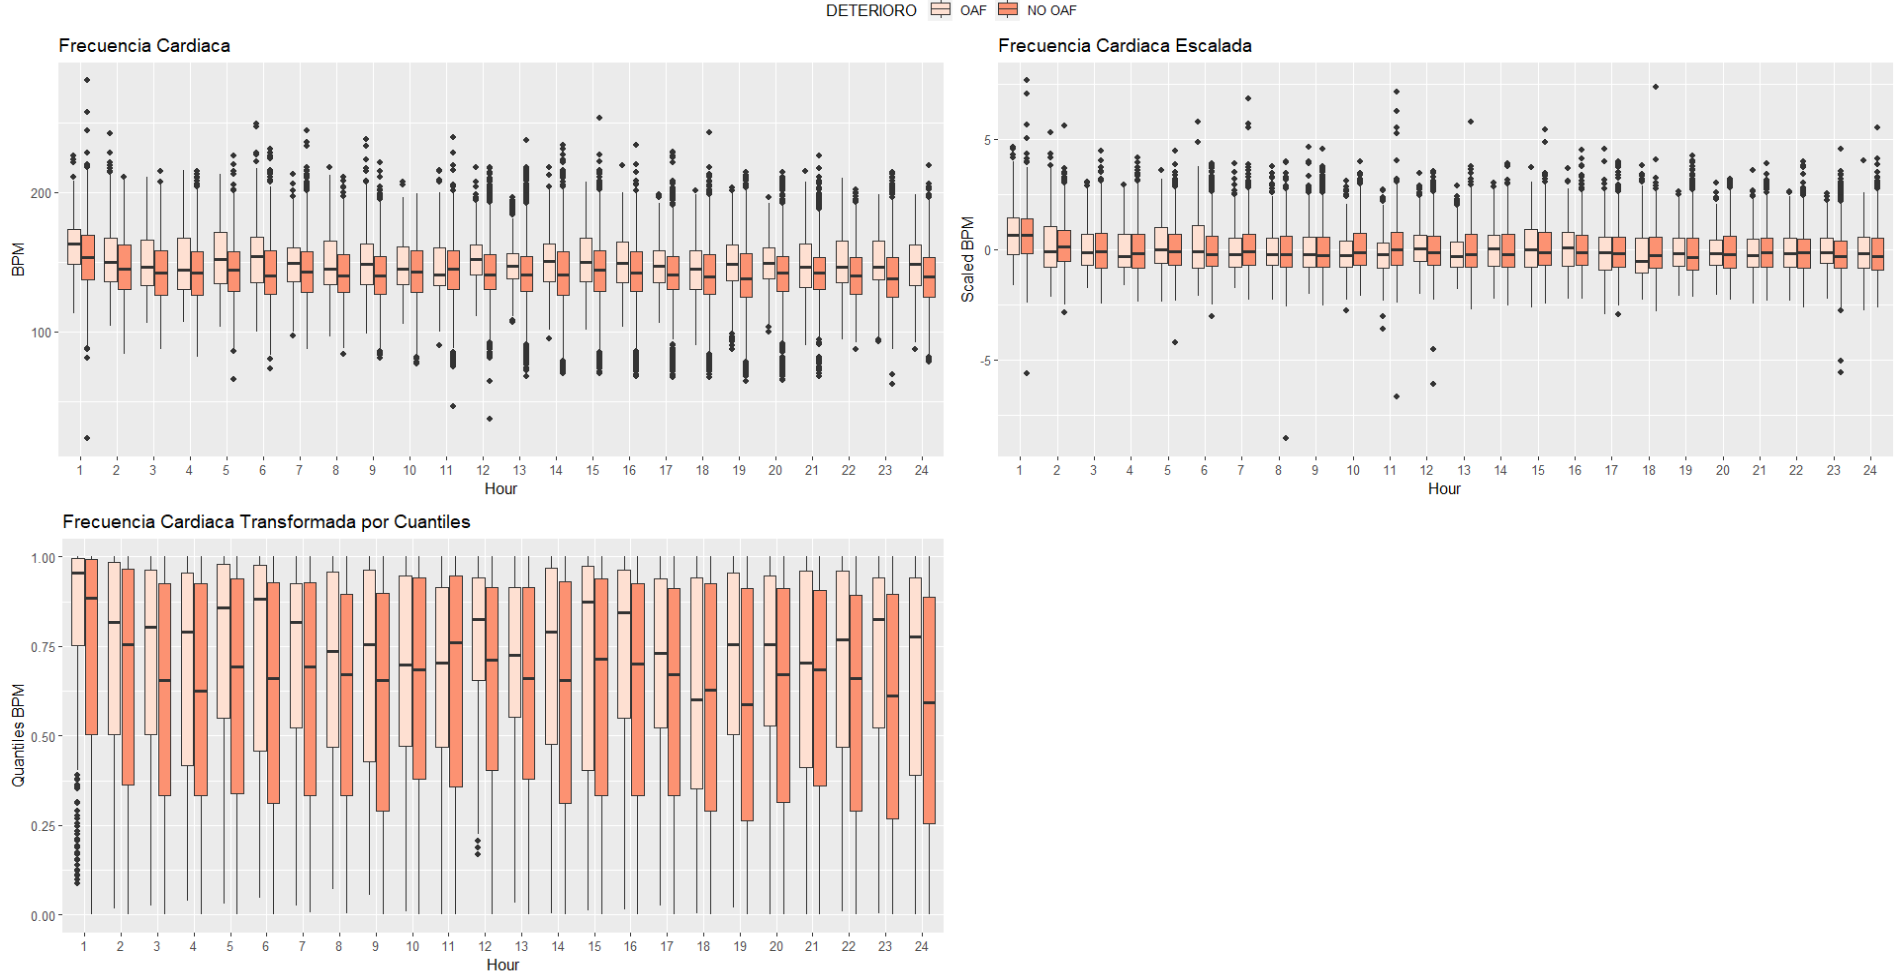
\includegraphics[scale = 0.68]{./img/fc-boxplot-mean.png}
    \caption{Media Horaria de la \textit{Frecuencia Cardíaca}, \textit{Frecuencia Cardíaca Escalada} y la \textit{Frecuencia Cardíaca Transformada por Cuantiles} entre pacientes que sufren DETERIORO y los que no}
    \label{fig:fc-boxplot-mean}
\end{figure}
\end{landscape}
\restoregeometry

\subsubsection{Saturación de Oxígeno}

A continuación, se muestra el análisis de la varianza realizado para la \textit{Saturación de O$_2$} y la \textit{Saturación de O$_2$ Escalada} entre pacientes que sufren DETERIORO y los que no. Se ha realizado el análisis de la varianza para cada una de las medias horarias. El resultado se muestra en la Tabla~\ref{tab:mean-SatO2}.

\begin{table}[H]
    \centering
    \begin{tabular}{|c|r|r|}
        \hline
        \textbf{Media Horaria} & \textbf{p-valor} & \textbf{p-valor escalada} \\
        \hline
        MEAN\_1 & 0.151 & 0.176 \\
        MEAN\_2 & 0.015 & 0.017 \\
        MEAN\_3 & 0.52 & 0.778 \\
        MEAN\_4 & 0.343 & 0.608 \\
        MEAN\_5 & 0.349 & 0.718 \\
        MEAN\_6 & 0.672 & 0.639 \\
        MEAN\_7 & 0.141 & 0.078 \\
        MEAN\_8 & 0.868 & 0.769 \\
        MEAN\_9 & 0.571 & 0.939 \\
        MEAN\_10 & 0.549 & 0.842 \\
        MEAN\_11 & 0.991 & 0.643 \\
        MEAN\_12 & 0.44 & 0.581 \\
        MEAN\_13 & 0.312 & 0.427 \\
        MEAN\_14 & 0.968 & 0.797 \\
        MEAN\_15 & 0.641 & 0.966 \\
        MEAN\_16 & 0.799 & 0.183 \\
        MEAN\_17 & 0.312 & 0.993 \\
        MEAN\_18 & 0.89 & 0.204 \\
        MEAN\_19 & 0.543 & 0.71 \\
        MEAN\_20 & 0.384 & 0.784 \\
        MEAN\_21 & 0.867 & 0.503 \\
        MEAN\_22 & 0.665 & 0.195 \\
        MEAN\_23 & 0.882 & 0.294 \\
        MEAN\_24 & 0.889 & 0.358 \\
        \hline
    \end{tabular}
    \caption{p-valor de la media horaria de la \textit{Saturación de O$_2$} entre pacientes que sufren OAF y los que no}\label{tab:mean-SatO2}
\end{table}

Al igual que en el apartado anterior el resultado es el siguiente mostrado en la Figura~\ref{fig:mean-SatO2}. La mayoría de las medias horarias no son significativas, por lo que no se puede rechazar la hipótesis nula. Esto significa que no hay diferencias significativas entre las medias horarias de la \textit{Saturación de O$_2$} entre pacientes que sufren DETERIORO y los que no.

Se puede observar como de manera general que a los pacientes que se les suministra OAF tienen una mayor \textit{Saturación de O$_2$} que los que no. Esto se puede observar en la Figura~\ref{fig:satO2-boxplot-mean}, aun así no se puede afirmar que esto tenga un efecto significativo de manera general en toda la monitorización del paciente.

La única media significativa menor que $\alpha = 0.05$ es la monitorizada en la hora $2$. Al igual que en el apartado anterior, esta situación va a causar a la hora de realizar el \textit{Estudio 2} se tendrán problemas a la hora de realizar un modelo de clasificación dónde los valores de monitorización de la \textit{Saturación de O$_2$} sean significativos a la hora de clasificar pacientes como DETERIORO o no.

{\color{blue} Hay algunas cosas que pueden estar influyendo en estos resultados "negativos": (1) El supuesto de varianzas iguales; (2) El supuesto de distribuciones normales. Ambos supuestos son los que conducen a la distribución t con n+m-2 grados de libertad. Por último, (3) la presencia de atípicos.}

\begin{figure}[H]
    \centering
    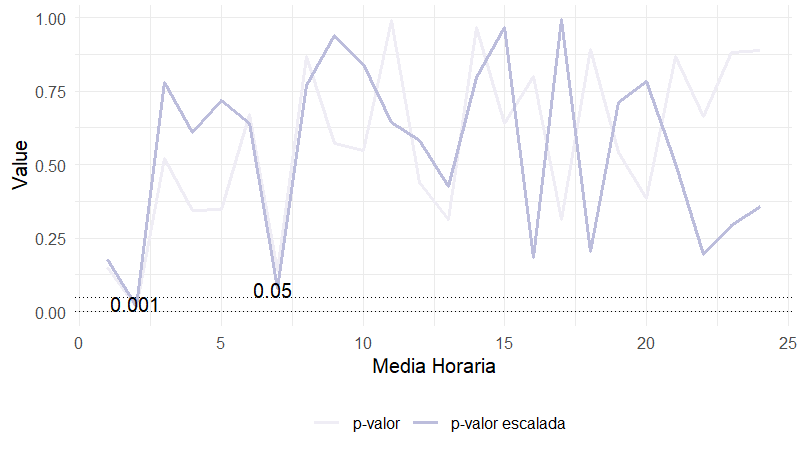
\includegraphics[scale = 1]{./img/mean-SatO2.png}
    \caption{p-valor de la media horaria de la \textit{Saturación de Oxígeno} entre pacientes que sufren DETERIORO y los que no}
    \label{fig:mean-SatO2}
\end{figure}

\newpage
\thispagestyle{empty}
% Se modifica la geometría (los márgenes) de la página y se coloca en formato horizontal:
\newgeometry{top=10mm, bottom=10mm, left=12mm, right=12mm}
\begin{landscape}
\begin{figure}[H]
    \centering
    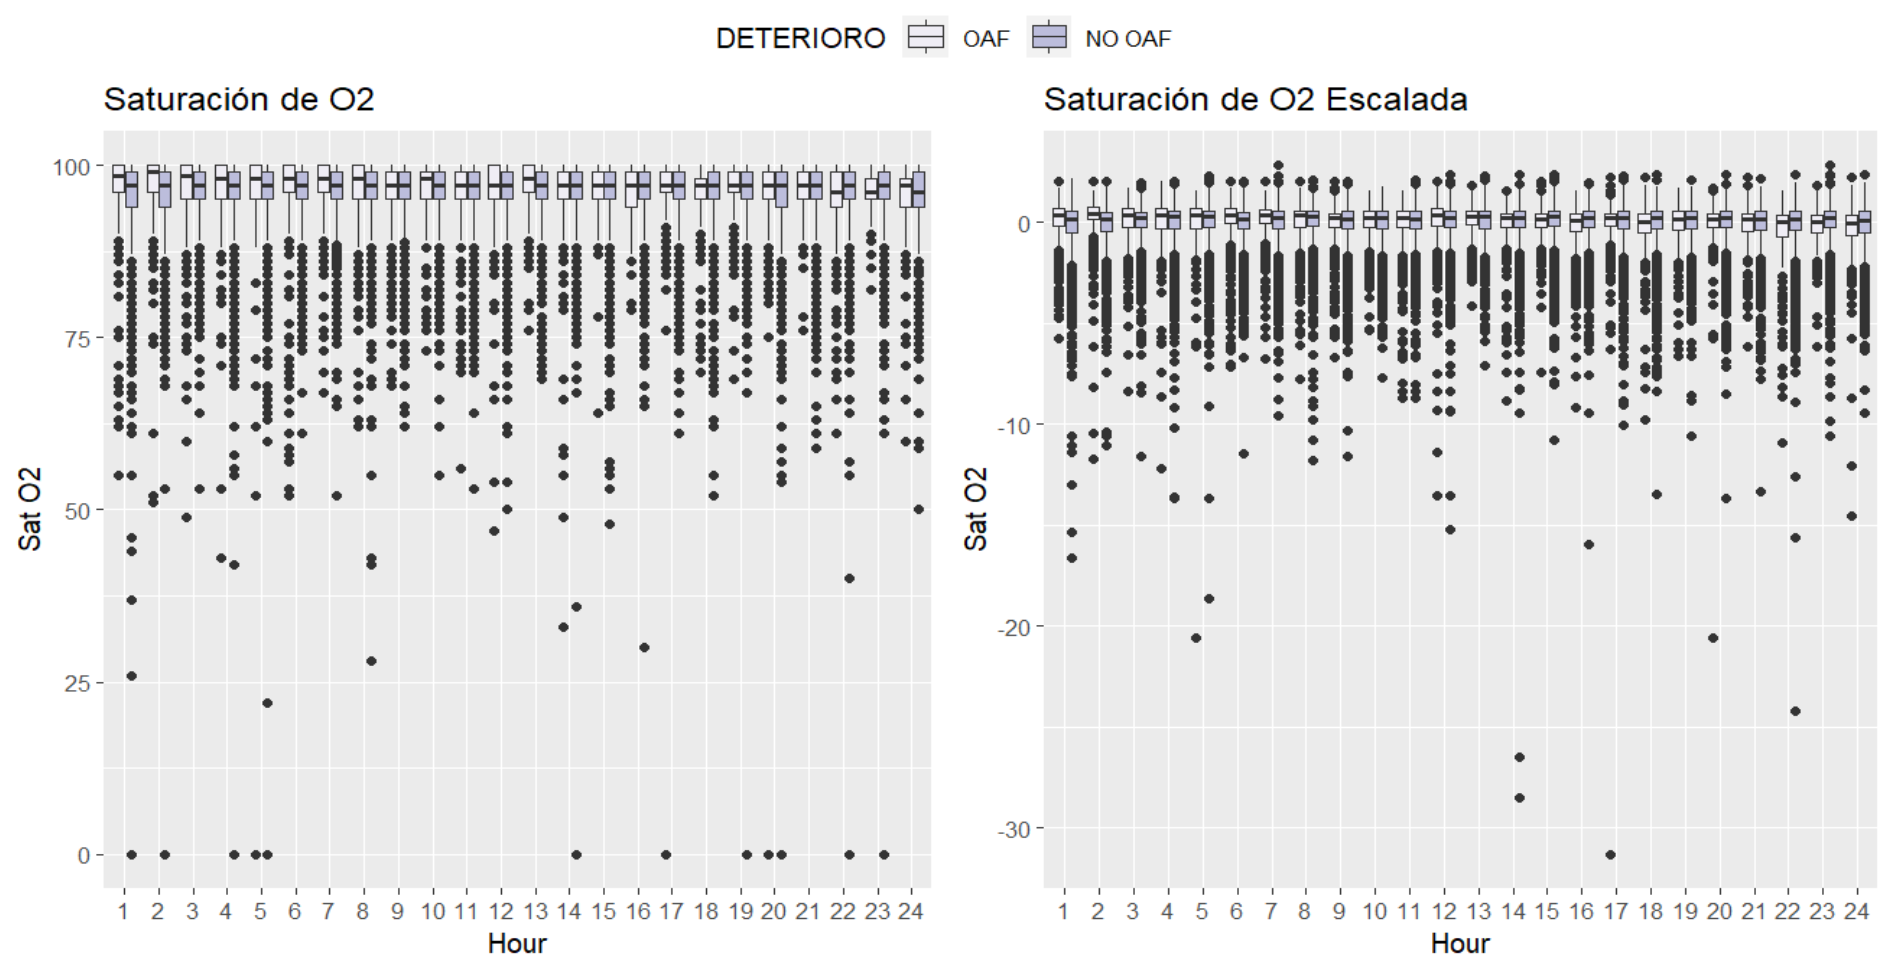
\includegraphics[scale = 0.68]{./img/satO2-boxplot-mean.png}
    \caption{Media Horaria de la \textit{Saturación de Oxígeno} y la \textit{Saturación de Oxígeno Escalada} entre pacientes que sufren DETERIORO y los que no}
    \label{fig:satO2-boxplot-mean}
\end{figure}
\end{landscape}
\restoregeometry


\subsection{Resultados: Estudio 2}\label{sec:resultados-estudio-1}

En esta sección de resultados, presentaremos los hallazgos obtenidos en el \textit{Estudio 2}. La sección se subdivide en cuatro subsecciones, y en cada una de ellas se mostrarán los siguientes resultados:

\begin{enumerate}
    \item Dendrograma de los clústeres obtenidos.
    \item Distribución de los clústeres obtenidos en función de las dos primeras componentes principales.
    \item Puntuación de Silhouette de los clústeres obtenidos.
    \item Dendrograma de los clústeres obtenidos según los pacientes que han experimentado OAF, junto con la tabla de contingencia.
    \item Clasificación mediante Random Forest de los clústeres según las variables \textit{Cuantitativas} y \textit{Cualitativas} de la Tabla~\ref{tabla:variables_estudio_final}, así como la Importancia de las cinco primeras variables.
    \item Clasificación Discriminante mediante Random Forest de los clústeres en función de los datos utilizados para generar los mismos clústeres (Raw Data, FAC, Peridiograma y FACC). Se mostrará la importancia para identificar qué datos contribuyen más en la clasificación entre los clústeres obtenidos.
    \item Cálculo de las medias de todos los valores empleados (Raw Data, FAC, Peridiograma y FACC) entre todos los pacientes, y diagrama de sus valores por clústeres.
\end{enumerate}

\paragraph{Leyenda de los gráficos}

\begin{enumerate}
    \item \textbf{Frecuencia Cardíaca}: \textit{HR}.
    \item \textbf{Saturación de Oxígeno}: \textit{SpO2}.
    \item \textbf{Frecuencia Cardíaca Escalada}: \textit{HR\_scaled}.
    \item \textbf{Saturación de Oxígeno Escalada}: \textit{SpO2\_scaled}.
    \item \textbf{Frecuencia Cardíaca Transformada por Cuantiles}: \textit{HR\_quantile}.
\end{enumerate}


\subsubsection{Raw Data}

\paragraph{Dendrograma de los clústeres obtenidos}

\begin{figure}[H]
    \centering
    
    \subfigure[\textit{HR}]{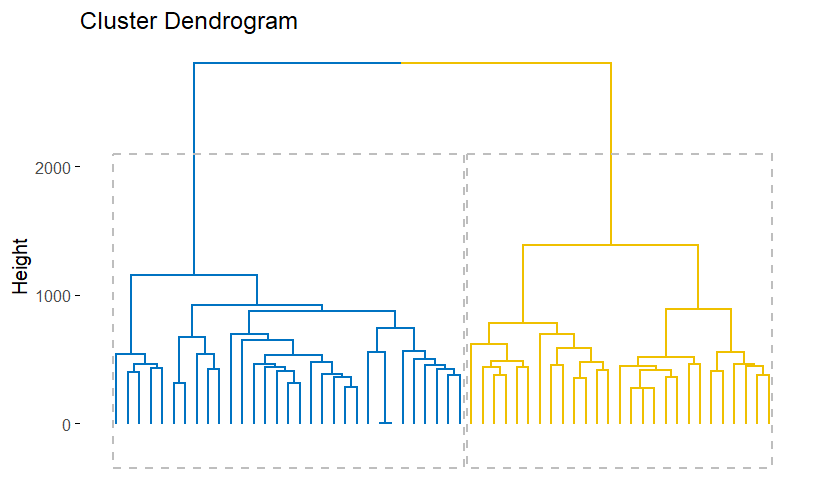
\includegraphics[width=0.45\textwidth]{img/01eucl-den.png}}
    \subfigure[\textit{HR\_scaled}]{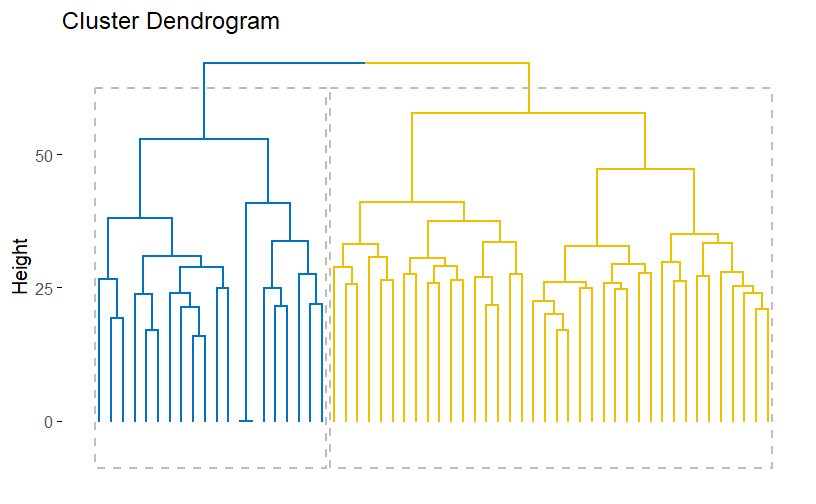
\includegraphics[width=0.45\textwidth]{img/02eucl-den.png}}
    \subfigure[\textit{HR\_quantile}]{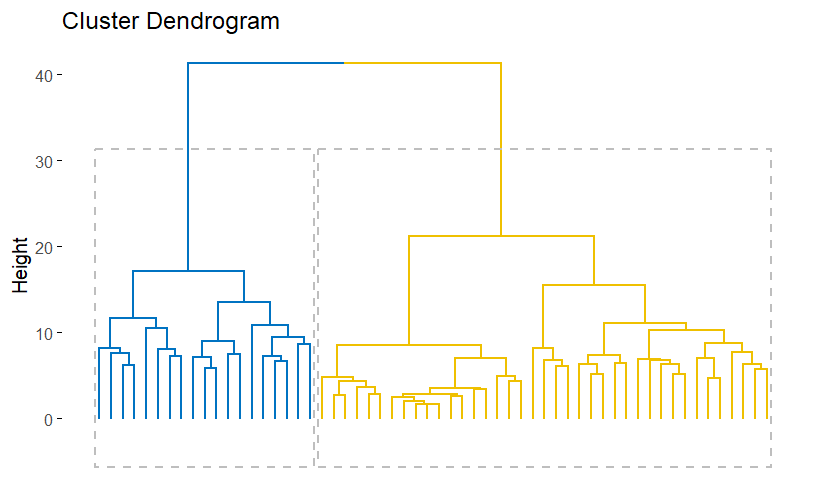
\includegraphics[width=0.5\textwidth]{img/03eucl-den.png}}
    \caption{Dendogramas de \textit{HR}, \textit{HR\_scaled} y \textit{HR\_quantile}}
    \label{fig:raw_data_den_fc}
\end{figure}

\begin{figure}[ht]
    \centering
    \subfigure[\textit{SpO2}]{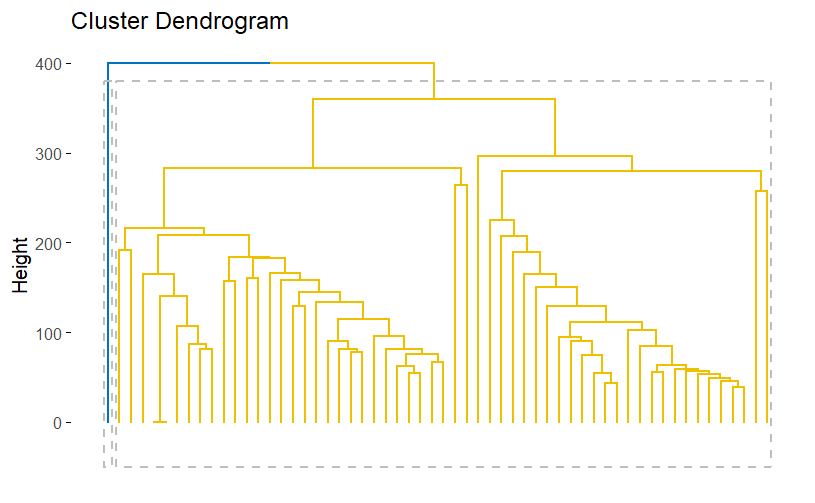
\includegraphics[width=0.5\textwidth]{img/04eucl-den.png}}\hfill
    \subfigure[\textit{SpO2\_scaled}]{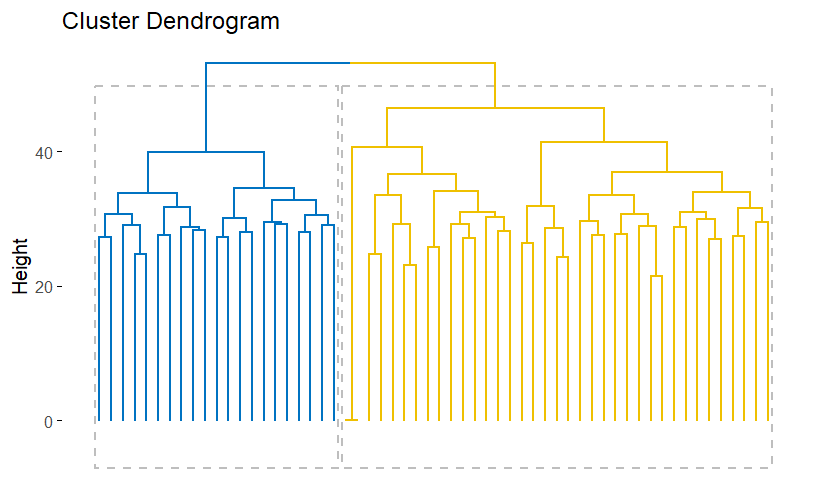
\includegraphics[width=0.5\textwidth]{img/05eucl-den.png}}
    \caption{Dendogramas de \textit{SpO2} y \textit{SpO2\_scaled}}\label{fig:raw_data_den_spo2}
\end{figure}

{\color{blue} Aunque el Silhouette sugiera dos clusters en la figura 5.5(a), es claro que el cluster azul es un dato atípico. Lo más sencillo es excluirlo del análisis y repetir el dendrograma.}

\paragraph{Distribución de los clústeres obtenidos en función de las dos primeras componentes principales}

\begin{figure}[H]
    \centering
    \subfigure[\textit{HR}]{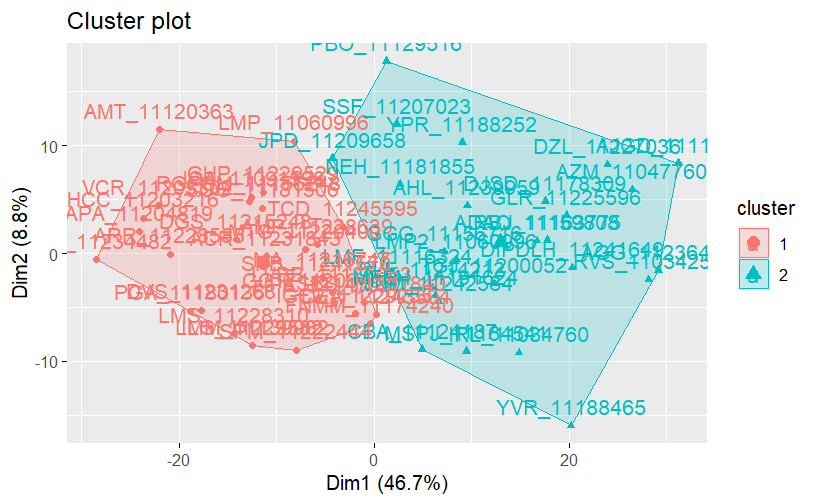
\includegraphics[width=0.45\textwidth]{img/01eucl-pc.png}}
    \subfigure[\textit{HR\_scaled}]{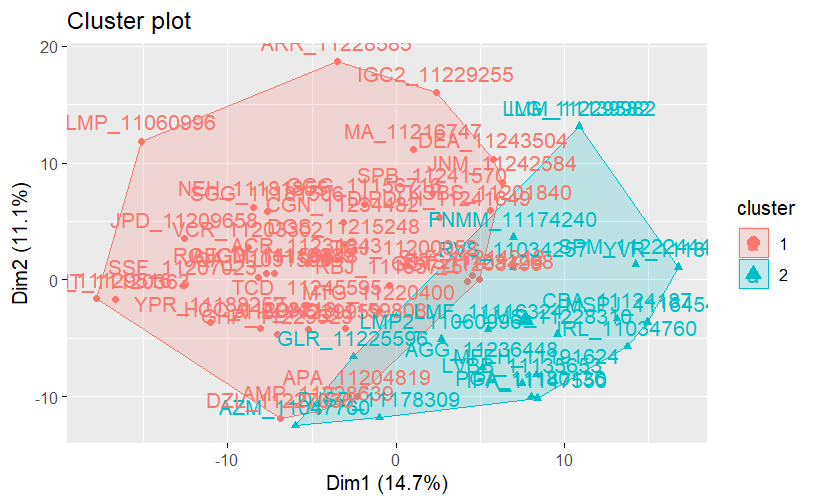
\includegraphics[width=0.45\textwidth]{img/02eucl-pc.png}}
    \subfigure[\textit{HR\_quantile}]{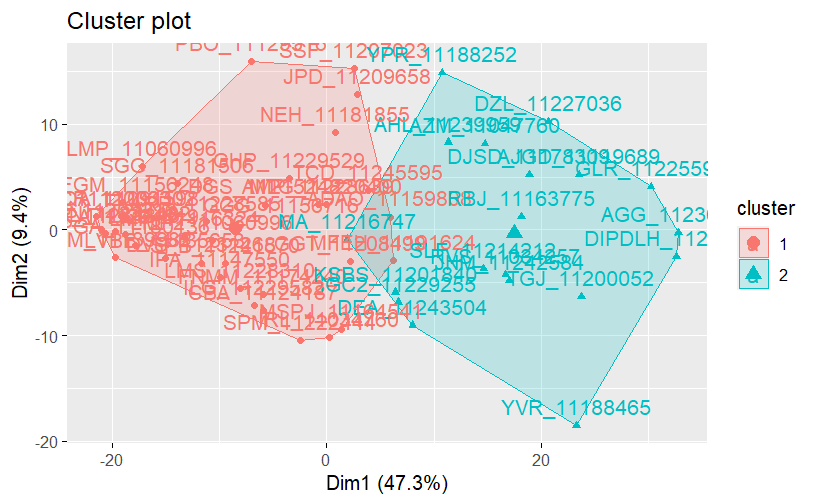
\includegraphics[width=0.5\textwidth]{img/03eucl-pc.png}}
    \caption{Cluster Plot de \textit{HR}, \textit{HR\_scaled} y \textit{HR\_quantile}}
    \label{fig:raw_data_pc_fc}
\end{figure}

\begin{figure}[ht]
    \centering
    \subfigure[\textit{SpO2}]{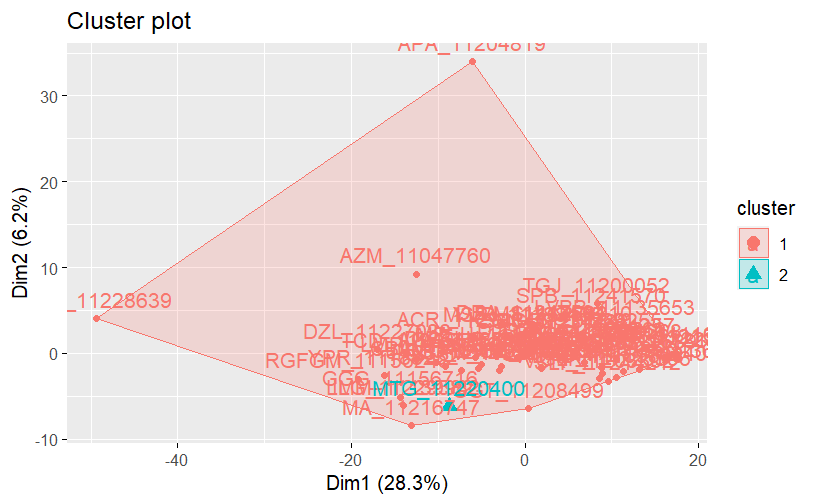
\includegraphics[width=0.5\textwidth]{img/04eucl-pc.png}}\hfill
    \subfigure[\textit{SpO2\_scaled}]{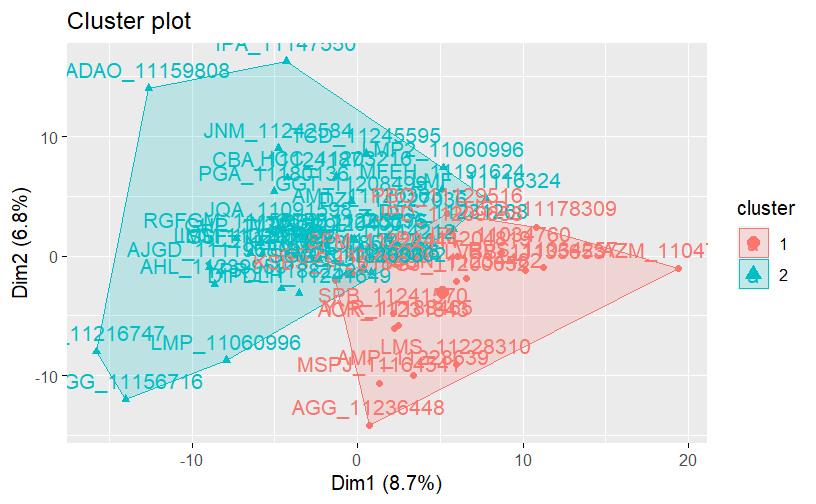
\includegraphics[width=0.5\textwidth]{img/05eucl-pc.png}}
    \caption{Cluster Plot de \textit{SpO2} y \textit{SpO2\_scaled}}\label{fig:raw_data_pc_spo2}
\end{figure}


\paragraph{Puntuación de Silhouette de los clústeres obtenidos}

\begin{figure}[H]
    \centering
    \subfigure[\textit{HR}]{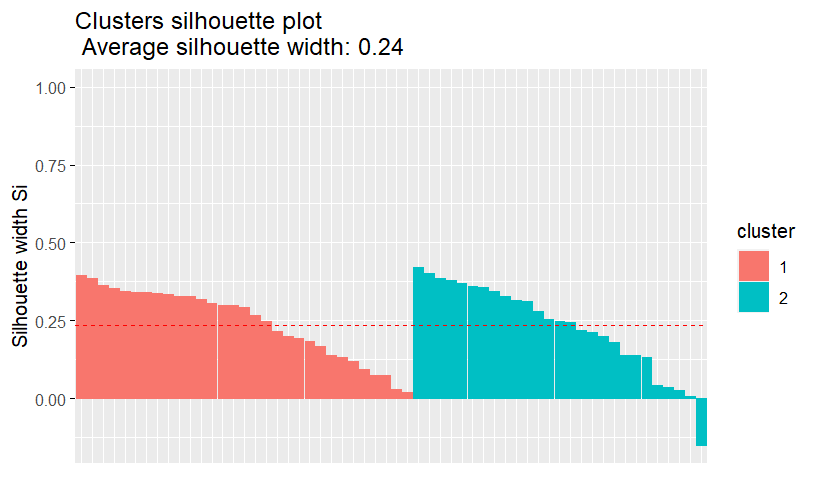
\includegraphics[width=0.45\textwidth]{img/01eucl-si.png}}
    \subfigure[\textit{HR\_scaled}]{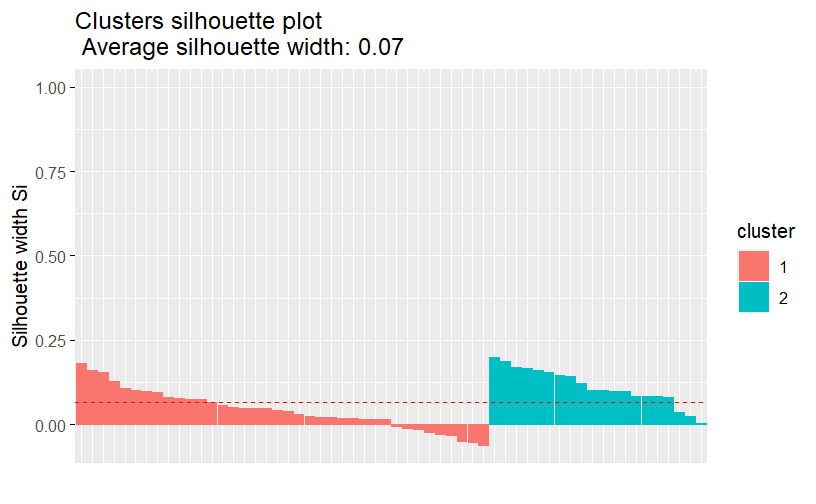
\includegraphics[width=0.45\textwidth]{img/02eucl-si.png}}
    \subfigure[\textit{HR\_quantile}]{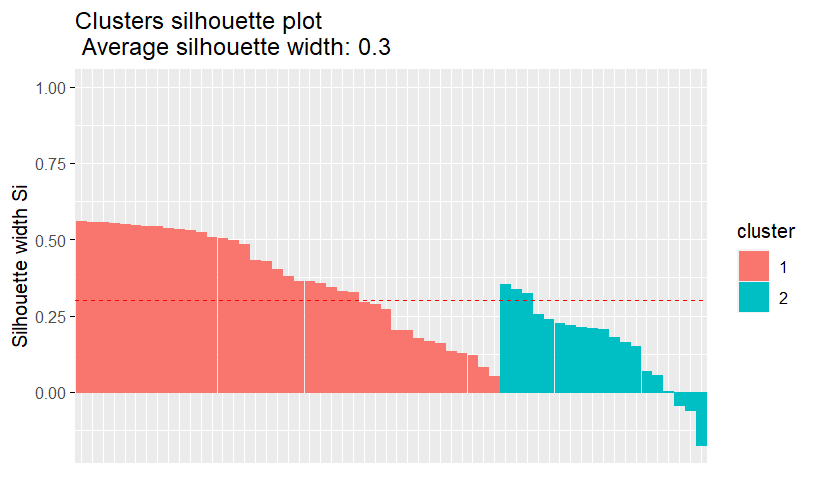
\includegraphics[width=0.5\textwidth]{img/03eucl-si.png}}
    \caption{Silhouette Plot de \textit{HR}, \textit{HR\_scaled} y \textit{HR\_quantile}}\label{fig:raw_data_si_fc}
\end{figure}

\begin{figure}[ht]
    \centering
    \subfigure[\textit{SpO2}]{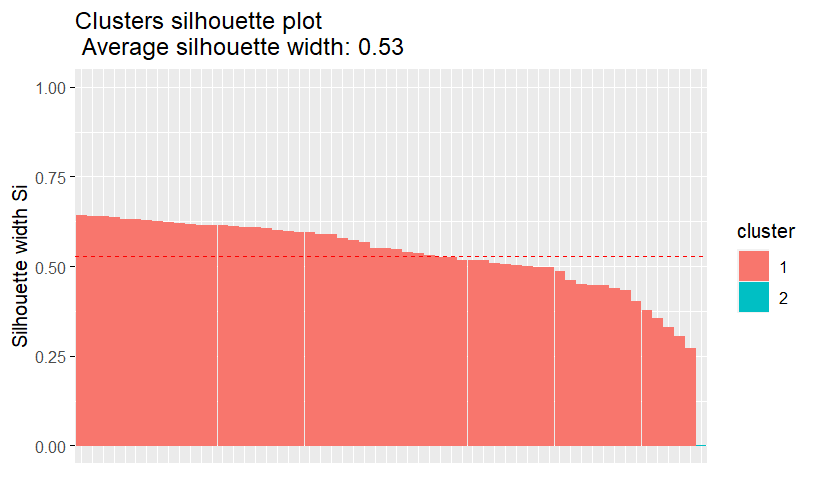
\includegraphics[width=0.5\textwidth]{img/04eucl-si.png}}\hfill
    \subfigure[\textit{SpO2\_scaled}]{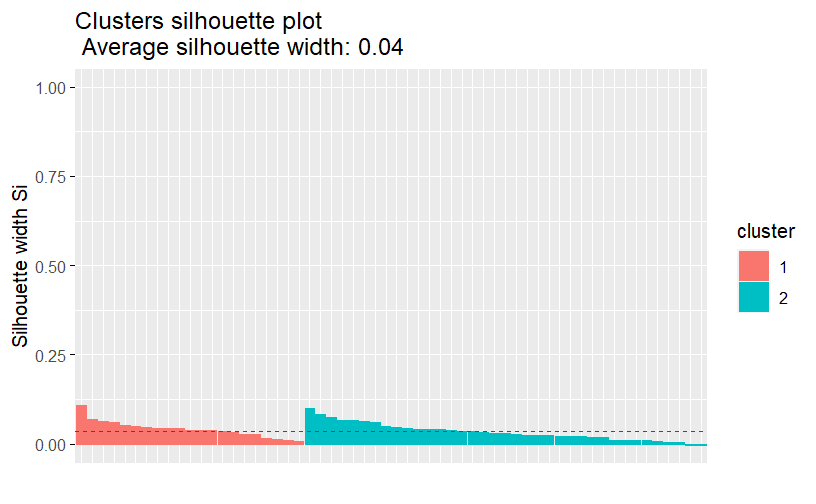
\includegraphics[width=0.5\textwidth]{img/05eucl-si.png}}
    \caption{Silhouette Plot de \textit{SpO2} y \textit{SpO2\_scaled}}\label{fig:raw_data_si_spo2}
\end{figure}


\subsubsection{FAC}

\subsubsection{Periodograma}

\subsubsection{FACC}